\documentclass[a4paper,10pt]{article}
\usepackage[vcentering,dvips]{geometry}

\newcommand{\linux}{\mbox{\sc LINUX}}
\newcommand{\awk}{\mbox{\sc awk}}
\newcommand{\sort}{\mbox{\sc sort}}

\newcommand {\articleTitle}{Informe Trabajo Pr\'actico 1}

% misc
\newcommand {\murl}[2]{\href{#1}{#2}}

% marcas / nombres de cosas usadas 
\usepackage[spanish]{babel}
\usepackage{graphicx}
\usepackage{graphics}
\usepackage[utf8]{inputenc}
\usepackage{subfigure}
\usepackage[pdftitle=\articleTitle
	pdfauthor={},
	pdfsubject={},
	pdfkeywords={} 
]{hyperref}

\usepackage{verbatim}
\usepackage{rotating}
% inclusion de codigo fuentes
\usepackage{listings}
\lstloadlanguages{c}


\author
{
	Pablo Giorgi,
	Santiago Perez De Rosso,
	Luciano Zemin
}

\date{Abril 2011}
% Title
\title{\articleTitle}

\begin{document}
\bibliographystyle{acm}
\maketitle

\tableofcontents

\section{Introducción}

En el presente informe se exponen las soluciones correspondientes al descifrado
de los archivos provistos por la c\'atedra y el an\'alisis de las cuestiones
planteadas en el punto 4 del Trabajo Pr\'actico 1.

\section{Descifrado de los archivos provistos por la c\'atedra}

Se desencriptaron los 6 archivos provistos por la c\'atedra
\emph{fun6AESCBC.wav}, \emph{fun6AESCFB.wav}, \emph{fun6AESOFB.wav},
\emph{fun6DESCBC.wav}, \emph{fun6DESOFB.wav} utilizando la clave \emph{sorpresa}
con el algoritmo y modo indicado en el nombre del archivo. Se obtuvo
el mismo fragmento de la canción \emph{El matador} de los \emph{Fabulosos Cadillacs}
en todos los casos.

\section{An\'alisis de las cuestiones planteadas en el punto 4 del Trabajo Pr\'actico 1}

\subsection{Ejercicio 4.1}
Para el primer punto, 4.1, se toma el archivo \emph{fa-do.wav} y se lo encripta
con DES en modo CBC, ECB, CFB y OFB y se analizan los resultados obtenidos.
Un resultado interesante para analizar es que as\'i como se ven bloques repetidos
en el archivo \emph{fa-do.wav} original tambi\'en se ven bloques repetidos en el 
resultado de encriptar el archivo original con DES ECB. Esta es una de las propiedades
del modo de operaci\'on ECB: bloques id\'enticos en el texto plano resultan en 
bloques id\'enticos en el texto cifrado. En la figura \ref{fig:41Original} se
muestran 2 fragmentos del archivo original donde se puede ver que se tienen bloques
repetidos. 
\begin{figure}
	\begin{center}
		\subfigure{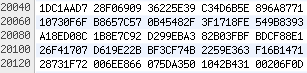
\includegraphics[scale=0.6]{../results/41/fadoRepetido1.png}}
		\subfigure{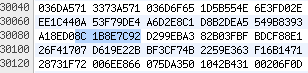
\includegraphics[scale=0.6]{../results/41/fadoRepetido2.png}}
	\end{center}
	\caption{Visualización del archivo original \emph{fa-do.wav} donde se pueden ver
		fragmentos repetidos.}
	\label{fig:41Original}
\end{figure}
\begin{figure}
	\begin{center}
		\subfigure{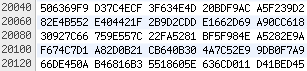
\includegraphics[scale=0.6]{../results/41/fadoECBRepetido1.png}}
		\subfigure{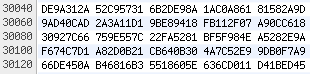
\includegraphics[scale=0.6]{../results/41/fadoECBRepetido2.png}}
	\end{center}
	\caption{Visualización del archivo \emph{fa-doDESECB.wav} donde se pueden ver
		fragmentos repetidos.}
	\label{fig:41ECB}
\end{figure}
En la figura \ref{fig:41ECB} se puede ver como el texto cifrado tiene tambi\'en bloques
repetidos en el mismo lugar. Otro resultado interesante a analizar es que la salida obtenida al usar
OFB y CFB tienen el primer bloque igual. En la figura \ref{fig:41OFBCFB} se puede ver
c\'omo el primer bloque que se encripta (el header no se encripta) resulta igual en ambos casos.
\begin{figure}
	\begin{center}
		\subfigure{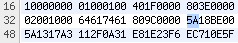
\includegraphics[scale=0.6]{../results/41/OFB.png}}
		\subfigure{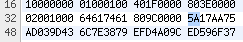
\includegraphics[scale=0.6]{../results/41/CFB.png}}
	\end{center}
	\caption{Visualización del archivo encriptado usando OFB y del archivo encriptado usando CFB.}
	\label{fig:41OFBCFB}
\end{figure}

\subsection{Ejercicio 4.2}
Idem ejercicio 4.1, a excepci\'on del cambio de tama\~no de la clave y vector de inicializaci\'on, los cuales se duplican. Por otro lado, el tama\~no del bloque de cifrado tambi\'en se modifica a ra\'iz de esto, a excepci\'on del modo CFB en el cual el tama\~no del bloque de cifrado siempre se mantiene en 8 bits utilizando la funci\'on de cifrado cfb8().

\subsection{Ejercicio 4.3}
La \'unica diferencia entre AES y DES es el tama\~no de la clave que se usa para encriptar y el tama\~no del bloque.\\
No se encuentran relaciones ni patrones comunes entre el archivo encriptado con AES y el mismo encriptado con DES.\\

\subsection{Ejercicio 4.4}
Para el punto 4.4 se toma el archivo de audio provisto por la c\'atedra \emph{la-fa.wav} y se lo
encripta usando DES
en modo ECB. Una vez que se obtiene el archivo encriptado se le modifica un bit, se lo desencripta y 
se compara el archivo obtenido con el original antes de ser encriptado.
Comparando a nivel byte ambos archivos se observa que son id\'enticos exceptuando 8 bytes, los cuales
son los que se corresponden con el bloque al que se le cambi\'o el bit.
\begin{table}
\begin{center}
\begin{tabular}{|c|c|c|}
\hline
Byte & Valor en el original [base 8] & Valor en el modificado [base 8]\\
\hline
\hline
61 & 222 & 120\\
62 & 352 & 374\\
63 & 151 & 77\\
64 & 322 & 120\\
65 & 162 & 265\\
66 & 274 & 42\\
67 & 273 & 304\\
68 & 251 & 16\\
\hline
\end{tabular}
\end{center}
\caption{Tabla donde se muestra el valor del byte indicado en el archivo original y en el archivo desencriptado despu\'es de la modificaci\'on.}
\label{table44a}
\end{table}
\begin{table}
\begin{center}
\begin{tabular}{|c|c|c|}
\hline
Byte & Valor en el original [base 8] & Valor en el modificado [base 8] \\
\hline
\hline
62 & 337 & 336\\
\hline
\end{tabular} 
\end{center}
\caption{Tabla donde se muestra el valor del byte indicado en el archivo encriptado original y en el archivo encriptado modificado.}
\label{table44b}
\end{table}
En el cuadro \ref{table44a} se muestra una comparaci\'on entre el archivo original y el archivo desencriptado a partir del que hab\'ia sufrido 
la modificaci\'on del bit. Se observa que la diferencia entre ambos es de exactamente 8 bytes consecutivos (1 bloque).
En el cuadro \ref{table44b} se muestra una comparaci\'on entre el archivo encriptado antes y despu\'es de ser modificado. Se observa que
el cambio es de un bit.
A partir de ambas tablas se puede concluir que un cambio de un bit en los archivos encriptados produce una modificaci\'on de un bloque completo
correspondiente al que se sufri\'o la modificaci\'on.
Tal comportamiento se debe a que los bloques se encriptan y desencriptan independientemente uno del otro, con lo cual, un cambio aislado en un bloque
no impacta de ninguna manera en los otros bloques. Esto se condice con la teor\'ia ya que una de las propiedades del
modo ECB es que si hay uno o m\'as bits con error en un bloque del texto cifrado esto solo afecta el descifrado de 
ese bloque en particular.

\subsection{Ejercicio 4.5}
Para el punto 4.5, a partir del archivo de audio provisto por la c\'atedra \emph{la-fa.wav}, se lo encripta usando DES
en modo CBC. Una vez que se obtiene el archivo encriptado se le modifica un bit, se lo desencripta y 
se compara el archivo obtenido con el original antes de ser encriptado.
Comparando a nivel byte ambos archivos se observa que son id\'enticos exceptuando 9 bytes. De estos 9 bytes,
8 son los que se corresponden con el bloque al que se le cambi\'o el bit, y el noveno es el byte del siguiente
bloque que se corresponde en posici\'on con el que se modific\'o en el bloque anterior.
\begin{table}
\begin{center}
\begin{tabular}{|c|c|c|}
\hline
Byte & Valor en el original [base 8] & Valor en el modificado [base 8]\\
\hline
\hline
141 & 31 & 222\\
142 & 316 & 52\\
143 & 356 & 42\\
144 & 345 & 262\\
145 & 4 & 300\\
146 & 377 & 322\\
147 & 46 & 344\\
148 & 30 & 144\\
156 & 146 & 147\\
\hline
\end{tabular}
\end{center}
\caption{Tabla donde se muestra el valor del byte indicado en el archivo original y en el archivo desencriptado despu\'es de la modificaci\'on.}
\label{table45a}
\end{table}
\begin{table}
\begin{center}
\begin{tabular}{|c|c|c|}
\hline
Byte & Valor en el original `[base 8] & Valor en el modificado [base 8]\\
\hline
\hline
148 & 60 & 61\\
\hline
\end{tabular}
\end{center}
\caption{Tabla donde se muestra el valor del byte indicado en el archivo encriptado original y en el archivo encriptado modificado.}
\label{table45b}
\end{table}
En el cuadro \ref{table45a} se muestra una comparaci\'on entre el archivo original y el archivo desencriptado a partir del que hab\'ia sufrido 
la modificaci\'on del bit. Se observa que la diferencia entre ambos es de exactamente 8 bytes consecutivos (1 bloque) y de un noveno byte del 
bloque siguiente, el cual es el que se encuentra en la posici\'on que se corresponde con el byte modificado del bloque anterior.
En el cuadro \ref{table45b} se muestra una comparaci\'on entre el archivo encriptado antes y despu\'es de ser modificado. Se observa que
el cambio es de un bit.
A partir de ambas tablas se puede concluir que un cambio de un bit en los archivos encriptados produce una modificaci\'on de un bloque completo
correspondiente al que se sufri\'o la modificaci\'on, y del byte del siguiente que se corresponde en posici\'on con el modificado en el archivo 
encriptado.
Tal comportamiento se debe a la forma en la que desencripta. Los 8 bytes del bloque que fue modificado en el archivo encriptado, se desencriptan
diferentes, dado que al entrar el texto cifrado modificado a la funci\'on de desencripci\'on, \'esta retorna un texto plano diferente. El noveno
byte que aparece diferente al original, se encuentra en el bloque siguiente al que fue modificado, y su existencia se debe a que una vez que la 
funci\'on de desencripci\'on desencript\'o el texto cifrado correspondiente al bloque aplica un \emph{OR} con el texto cifrado del bloque anterior, 
el cual ten\'ia un bit modificado. Es por tal motivo que el bloque siguiente aparece con un byte diferente al original.
Esta es una de las propiedades del modo de operaci\'on CBC: un solo bit con error en el bloque cifrado $ c_{j} $ afecta
el descifrado de los bloques $ c_{j} $ y $ c_{j +1} $. Aparte de esto el texto plano recuperado $ x_{j + 1} $ tiene
errores en el mismo lugar que $ c_{j} $ tuvo. 
\subsection{Ejercicio 4.6}
Para el punto 4.6 se toma el fragmento de la canci\'on \emph{El Matador} de los \emph{Fabulosos Cadillacs} 
obtenido a partir de desencriptar uno de los archivos provistos por la c\'atedra.
Dado que la cantidad de bloques que se corrompen al romper un bit de lo que est\'a encriptado y luego
desencriptarlo, es $1 + \frac{n}{r}$, donde $n$ es el tamaño de la clave $K$ ($128$ bits en AES, 64 en DES) y $r$ es el tamaño de
bloque de CFB (tamaño de bloque considerado en el conteo de bloques corruptos), en este caso 8 bits (la funcion de cifrado utilizada es CFB8). Esto se debe a que un error en un bloque cifrado de CFB necesita r shifteos para desaparecer y dejar de propagar el error introducido en 1 bit. Entonces, la cantidad de bytes corruptos en DES debe ser $1 + 64/8 = 9$.
En el cuadro \ref{table46} se puede ver los bytes en los que difieren el archivo original y el desencriptado a partir
del encriptado modificado.
\begin{table}
\begin{center}
\begin{tabular}{|c|c|c|}
\hline
Byte & Valor en el original [base 8] & Valor en el modificado [base 8]\\
\hline
\hline
1874216 & 377 & 376 \\
1874217 & 254 & 270 \\
1874218 & 363 & 26 \\
1874219 & 354 & 144 \\
1874220 & 366 & 160 \\
1874221 & 102 & 15 \\
1874222 & 344 & 277 \\
1874223 & 0 & 236 \\
1874224 & 361 & 20 \\
\hline
\end{tabular}
\end{center}
\caption{Tabla donde se muestra el valor del byte indicado en el archivo encriptado original y en el archivo encriptado modificado.}
\label{table46}
\end{table}

\subsection{Ejercicio 4.7}

Para el punto 4.7 se considera el mismo archivo que para el ejercicio 4.6. La diferencia es que para el caso de usar
AES (AES128) la cantidad de bytes corruptos debe ser $ 1 + \frac{128}{8} = 17$. En el cuadro \ref{table47} se puede ver los bytes en los que difieren el archivo original y el desencriptado a partir
del encriptado modificado.
\begin{table}
\begin{center}
\begin{tabular}{|c|c|c|}
\hline
Byte & Valor en el original [base 8] & Valor en el modificado [base 8]\\
\hline
\hline
1817504 & 357 & 356 \\
1817505 & 40 & 225 \\
1817506 & 365 & 346 \\
1817507 & 246 & 245 \\
1817508 & 27 & 360 \\
1817509 & 143 & 324 \\
1817510 & 6 & 333 \\
1817511 & 311 & 267\\
1817512 & 17 & 76\\
1817513 & 362 & 255\\
1817514 & 14 & 370\\
1817515 & 353 & 132 \\
1817516 & 370 & 271\\
1817517 & 4 & 240\\
1817518 & 13 & 25\\
1817519 & 12 & 224\\
1817520 & 360 & 376\\
\hline
\end{tabular}
\end{center}
\caption{Tabla donde se muestra el valor del byte indicado en el archivo encriptado original y en el archivo encriptado modificado.}
\label{table47}
\end{table}

\subsection{Ejercicio 4.8}
Respecto al punto 4.8 se encripta el archivo \emph{fa-do.wav} utilizando DES OFB.
Se cambia un bit del texto cifrado (en el byte 4673) y se desencripta. Al comparar
el archivo original con el desencriptado corriendo
\begin{lstlisting}
cmp -l results/48/fa-do.wav results/48/fa-doDesencriptado.wav 
\end{lstlisting}
se obtiene 
\begin{lstlisting}
 4673 121 120
\end{lstlisting}
Esto indica que en el byte 4673 hay una diferencia de un bit y que s\'olo es \'esta la diferencia.
\begin{figure}
	\begin{center}
		\subfigure{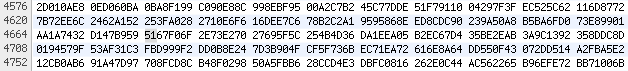
\includegraphics[scale=0.6]{../results/48/fa-do.png}}
		\subfigure{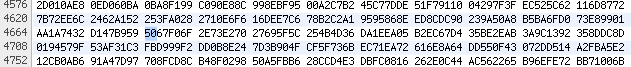
\includegraphics[scale=0.6]{../results/48/fa-doModificado.png}}
	\end{center}
	\caption{Visualización del archivo original \emph{fa-da.wav} y del archivo obtenido 
		al desencriptar el cifrado modificado con la diferencia marcada.}
	\label{fig:48}
\end{figure}
Esto se condice con la teor\'ia ya que una de las caracter\'isticas de OFB es que si
hay uno o m\'as bits con errores en cualquier caracter $ c_{j} $ del texto cifrado s\'olo afecta el descifrado de ese caracter. Y dado el texto plano se van a ver
los bits complementados respecto al original sin error en las mismas posiciones donde 
se cambiaron los bits del texto cifrado. En la figura \ref{fig:48} se muestra una 
parte del archivo original \emph{fa-do.wav} y el archivo obtenido al desencriptar
el cifrado alterado donde se puede ver la diferencia.

\subsection{Ejercicio 4.9}
Finalmente, respecto al punto 4.9 se utiliza DES con el m\'etodo ECB para encriptar
los archivos \emph{do-fa.wav} y \emph{si-mi.wav} con el objetivo de comparar la salida
con el archivo \emph{incogDES.wav} y as\'i determinar qu\'e notas tiene el archivo
\emph{incogDES.wav}. Analizando los resultados con el Audacity se puede ver en la figura
\ref{fig:DESAudacityCmp} c\'omo la onda correspondiente al archivo \emph{si-mi.wav} encriptado es igual a la correspondiente al archivo \emph{incogDES.wav} para la primera parte, y luego, la onda correspondiente al archivo \emph{do-fa.wav} encriptado es igual a la correspondiente al archivo \emph{incogDES.wav} para la \'ultima parte. De esta forma,
sin desencriptar el archivo \emph{incogDES.wav} se puede decir que \'este posee las notas \emph{si} y \emph{fa}.
Desencriptando el archivo se verifica empíricamente lo supuesto.\\
\begin{figure}
	\begin{center}
		\subfigure{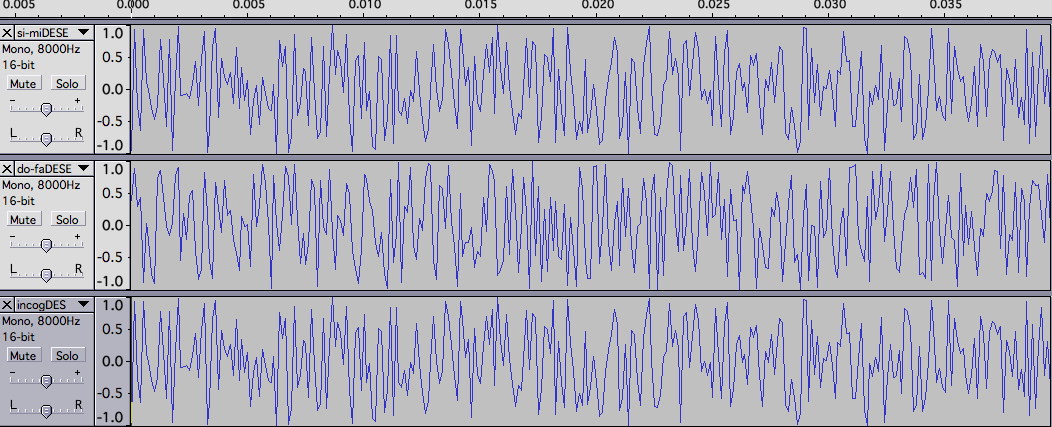
\includegraphics[scale=0.4]{../results/49/DES/audacityCmp1.png}}
		\subfigure{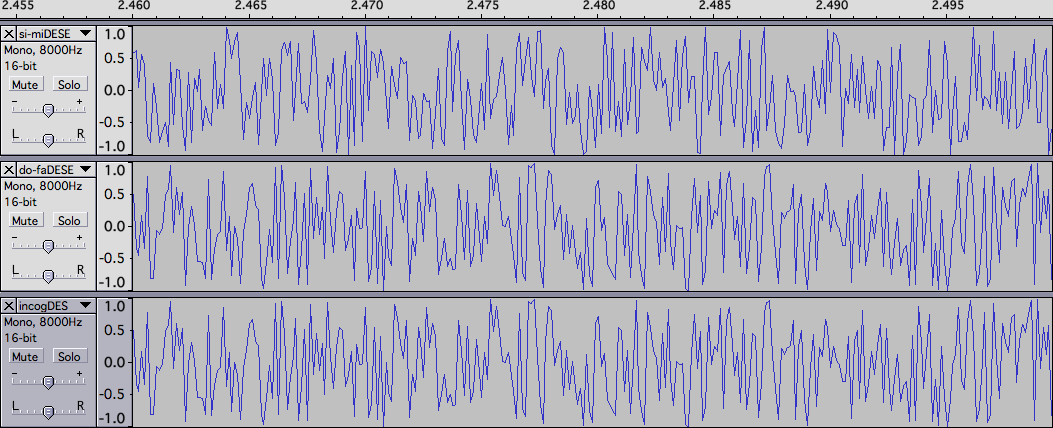
\includegraphics[scale=0.4]{../results/49/DES/audacityCmp2.png}}
	\end{center}
	\caption{Visualización de los archivos \emph{si-miDESECB.wav}, \emph{do-faDESECB.wav} y
		\emph{incogDES.wav} en el Audacity.}
	\label{fig:DESAudacityCmp}
\end{figure}

Lo mismo se realiza para el caso donde se debe utilizar AES con el m\'etodo ECB para encriptar
los archivos \emph{fa-do.wav} y \emph{mi-si.wav} con el objetivo de comparar la salida
con el archivo \emph{incogAES.wav} y as\'i determinar qu\'e notas tiene el archivo
\emph{incogAES.wav}. Sin desencriptar el archivo \emph{incogAES.wav} se puede decir que \'este
posee las notas \emph{fa} y \emph{si}. En la figura \ref{fig:AESAudacityCmp} se ven las ondas
pertinentes con el Audacity. Desencriptando el archivo se verifica empíricamente lo supuesto.
\begin{figure}
	\begin{center}
		\subfigure{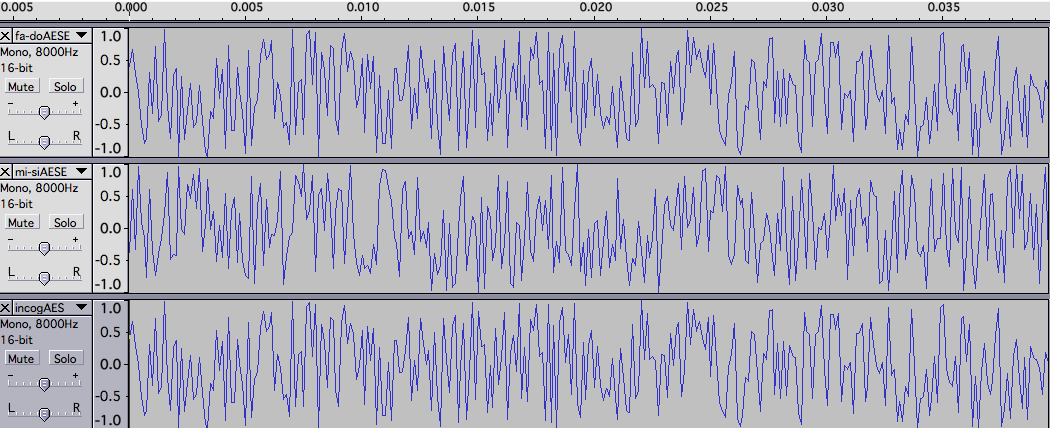
\includegraphics[scale=0.4]{../results/49/AES/audacityCmp1.png}}
		\subfigure{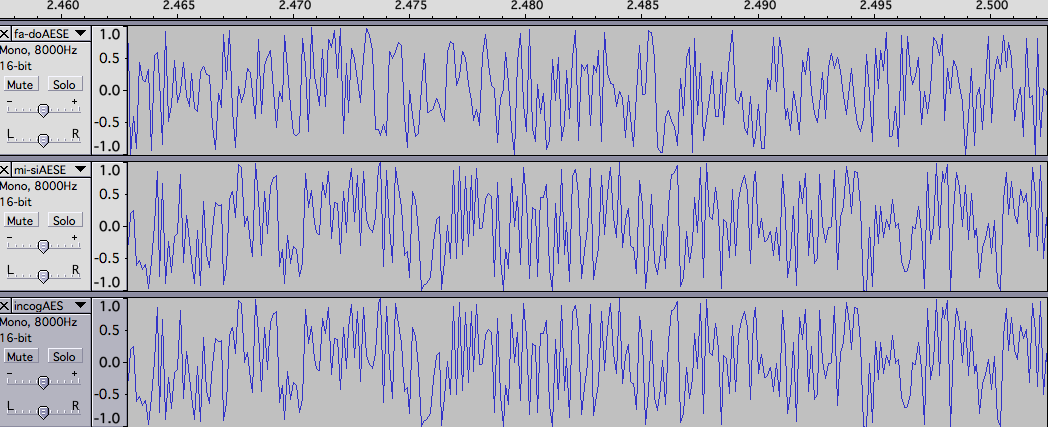
\includegraphics[scale=0.4]{../results/49/AES/audacityCmp2.png}}
	\end{center}
	\caption{Visualización de los archivos \emph{fa-daAESECB.wav}, \emph{mi-siAESECB.wav} y
		\emph{incogAES.wav} en el Audacity.}
	\label{fig:AESAudacityCmp}
\end{figure}
\end{document}
